\documentclass{beamer}
\usepackage[T1]{fontenc}
\usepackage[utf8]{inputenc}
\usepackage{graphicx}
\usepackage[normalem]{ulem}
\usepackage{xmpmulti}
\usepackage{marvosym}
% \usepackage[dvipsnames]{xcolor}
% \usepackage{enumitem}


\newcommand{\emphh}[1]{\textcolor{blue}{\emph{#1}}}
\newcommand{\hilite}[1]{\emphh{#1}}
\title{Planar Graphs in Blowups of Fans}

\newcommand{\verteq}{\rotatebox{90}{$\equiv$}}

\author{}
\author{\only<1>{%
  Vida~Dujmović \and
  Gwenaël~Joret \and
  Piotr~Micek \newline \and
  Pat Morin \and
  David R. Wood}%
  \only<2>{%
    Gwenaël~Joret \and
    Pat Morin \and
    David R. Wood \newline \and
    Vida~Dujmović \and
    Piotr~Micek}%
     \\[3ex]
  \only<1>{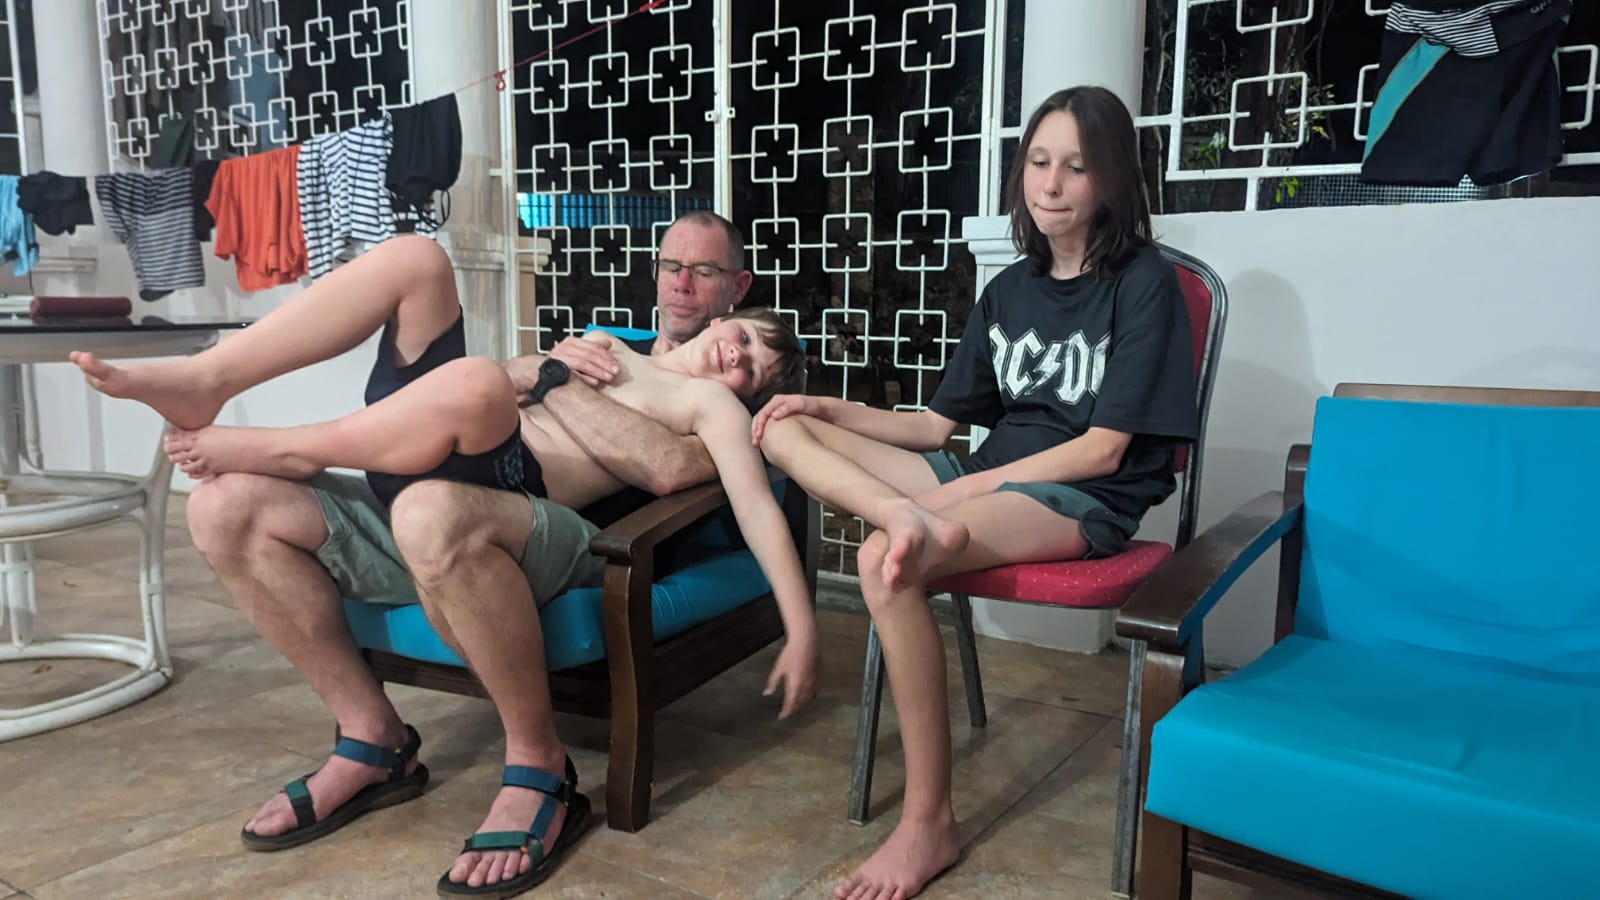
\includegraphics[height=.428\textheight]{images/pat-and-kids}\\(How we started)}
  %
  \only<2>{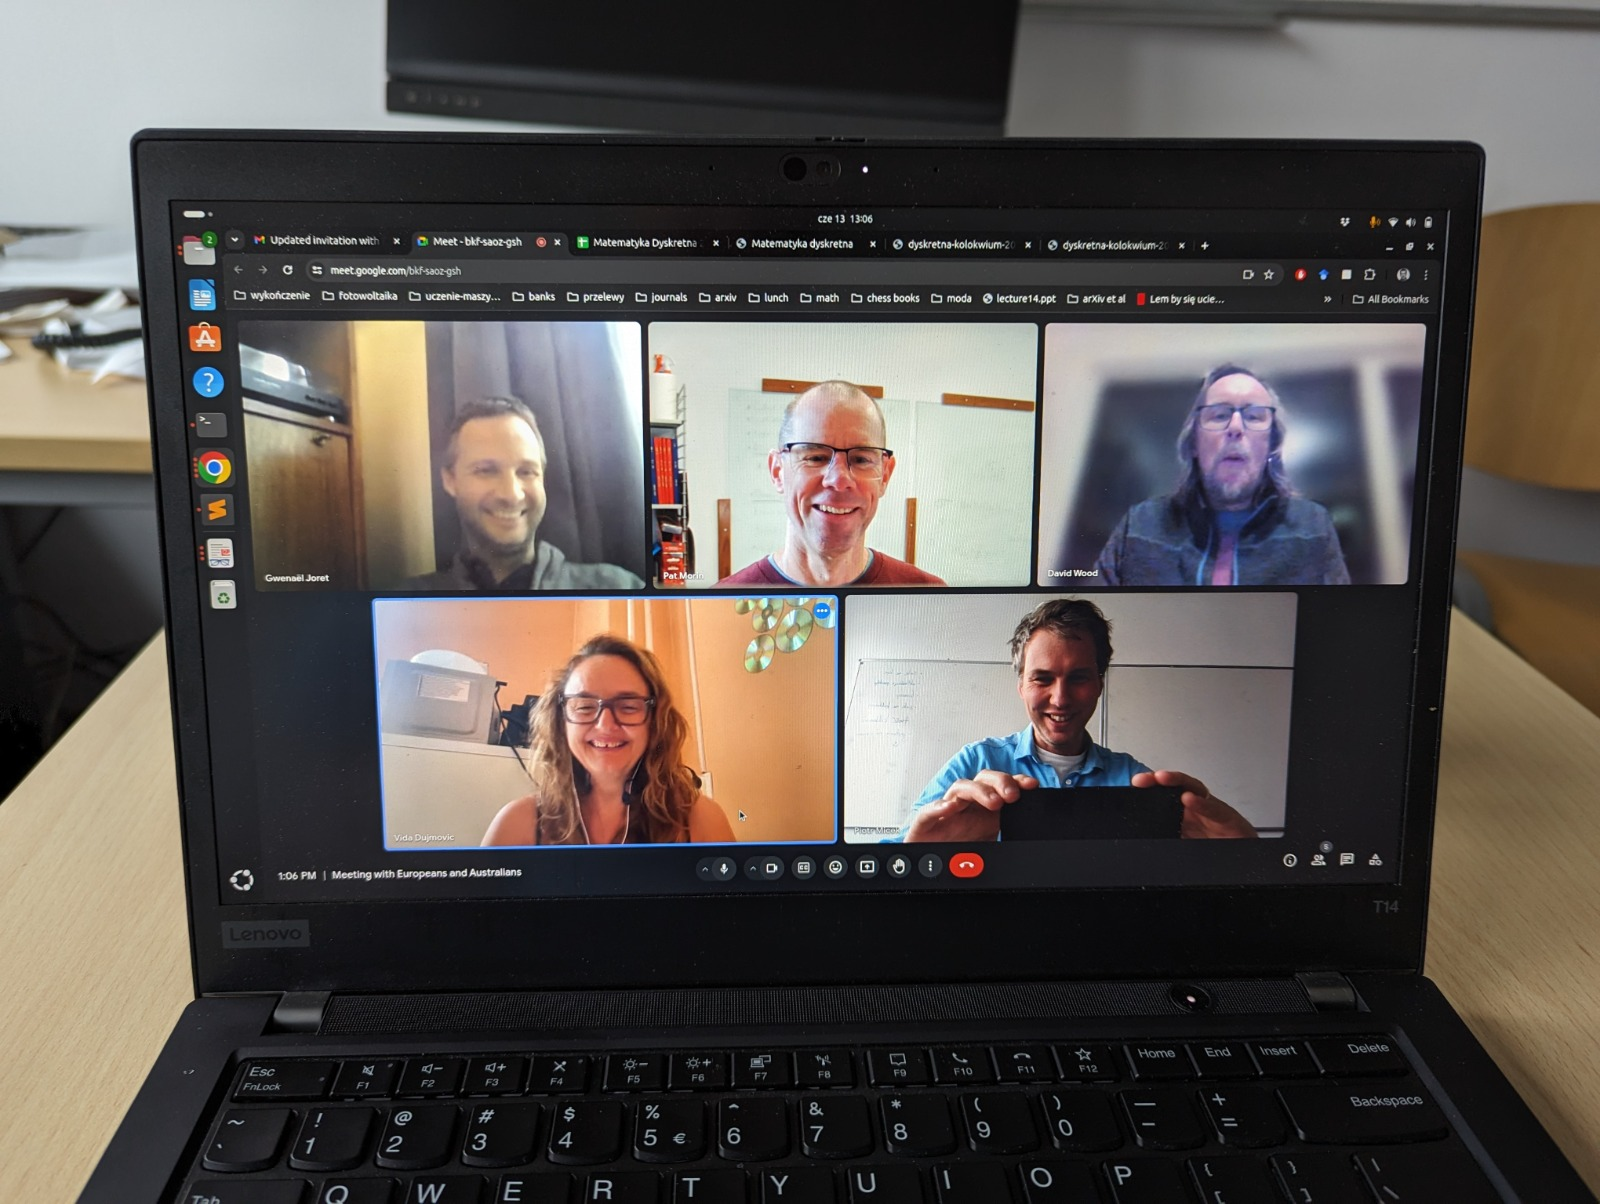
\includegraphics[height=.428\textheight]{images/authors}\\(How we finished)}%
}
\date{}

\setbeameroption{hide notes} % Only slides
%\setbeameroption{show only notes} % Only notes
% \setbeameroption{show notes on second screen=right} % Both


% \DeclareMathOperator{\tw}{tw}
% \DeclareMathOperator{\td}{td}
% \DeclareMathOperator{\wcol}{wcol}
% \DeclareMathOperator{\lvr}{\chi_{\ell-\mathrm{vr}}}
% \DeclareMathOperator{\pcn}{\chi_{p}}
\newcommand{\N}{\mathbb{N}}
\begin{document}

\begin{frame}
  % \begin{center}
    \maketitle
  % \end{center}
\end{frame}

\begin{frame}
  \frametitle{Outline}

  \begin{itemize}
    \item Theorem statement
    \item Some related work
    \item Proof sketch
  \end{itemize}
\end{frame}


\begin{frame}
  \frametitle{Lipton-Tarjan Planar Separator Theorem}
  \framesubtitle{Lipton-Tarjan 1979}

  \begin{center}
    \only<1>{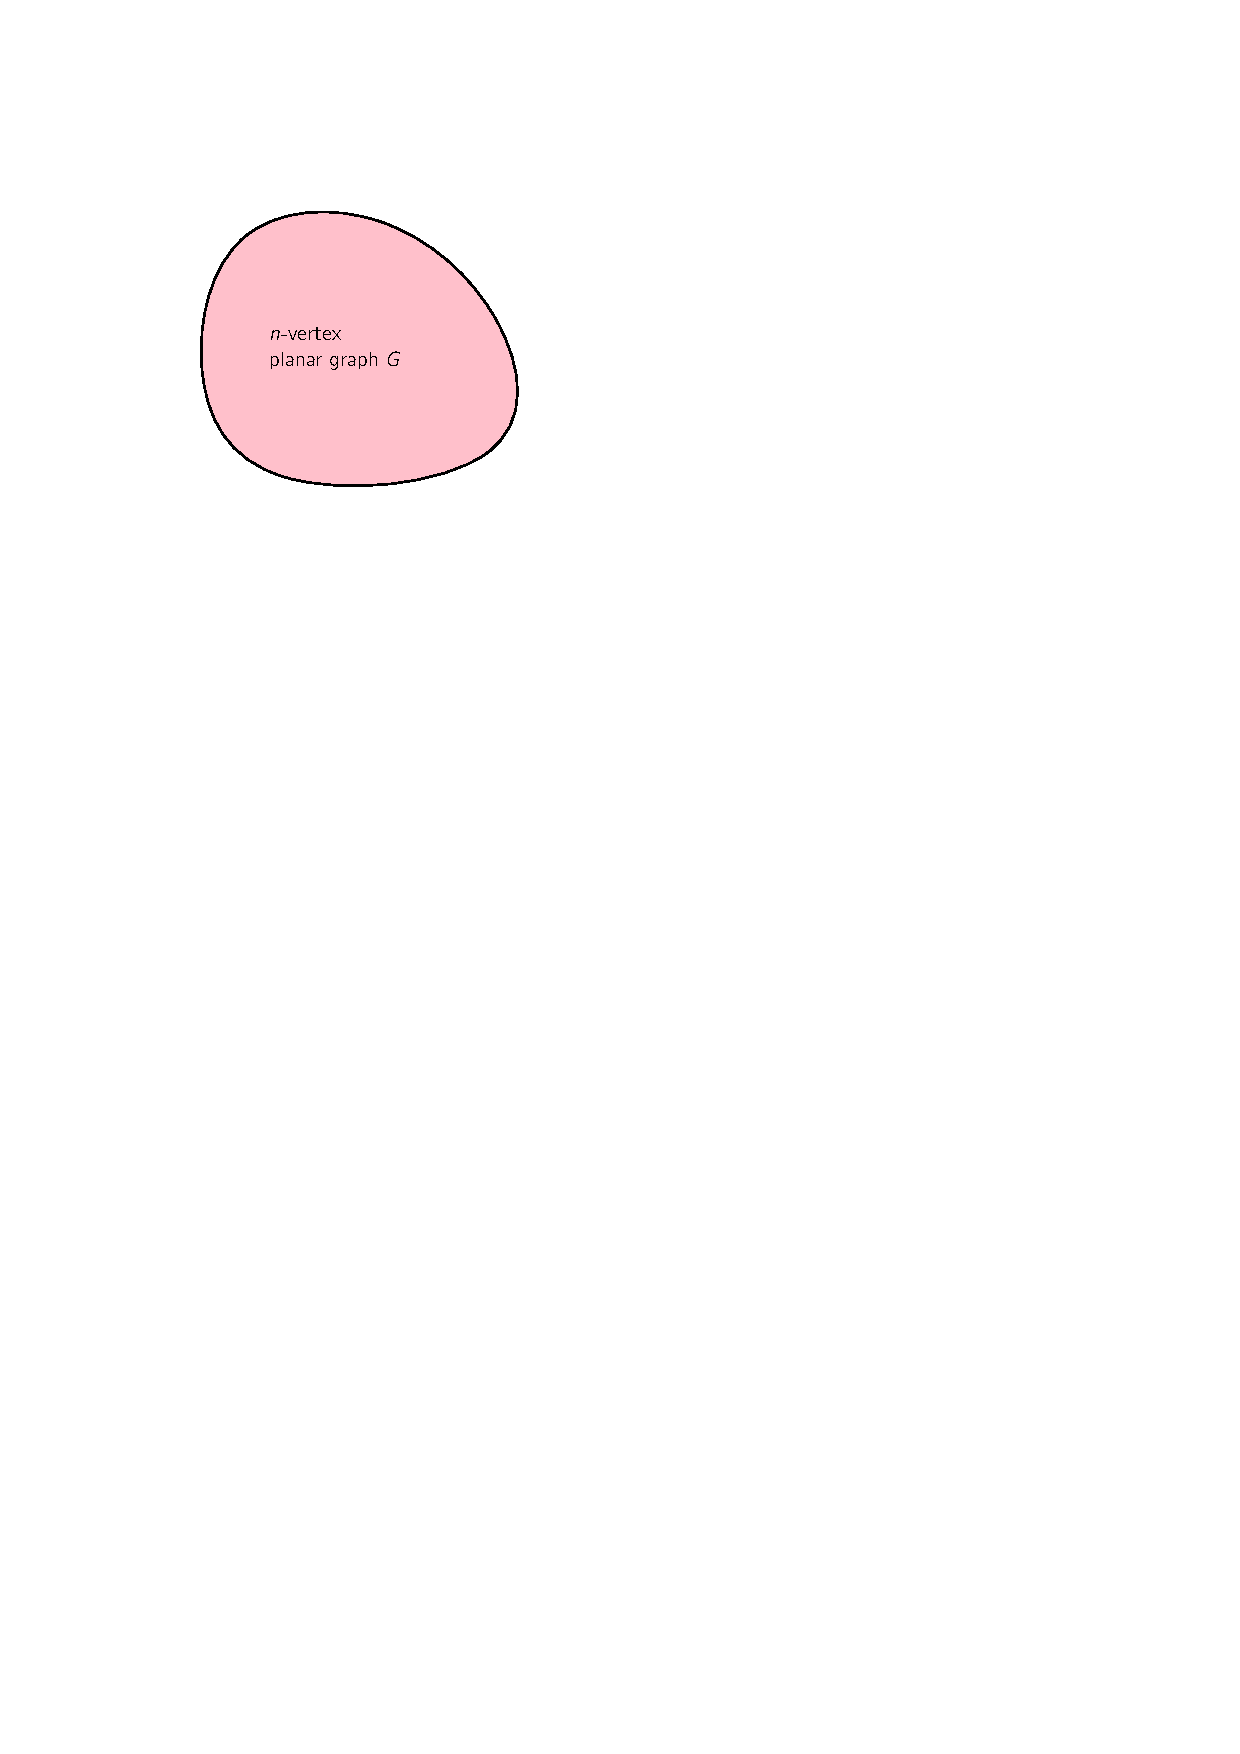
\includegraphics[page=1]{figs/lipton-tarjan-star}}%
    \only<2>{\includegraphics[page=2]{figs/lipton-tarjan-star}}%
    \only<3>{\includegraphics[page=3]{figs/lipton-tarjan-star}}%
    \only<4>{\includegraphics[page=4]{figs/lipton-tarjan-star}}%
    \only<5>{\includegraphics[page=5]{figs/lipton-tarjan-star}}%
    \only<6>{\includegraphics[page=6]{figs/lipton-tarjan-star}}%
    \only<7>{\includegraphics[page=7]{figs/lipton-tarjan-star}}%
    \only<8>{\includegraphics[page=8]{figs/lipton-tarjan-star}}%
    \only<9>{\includegraphics[page=9]{figs/lipton-tarjan-star}}%
    \only<10>{\includegraphics[page=10]{figs/lipton-tarjan-star}}%
    \only<11>{\includegraphics[page=11]{figs/lipton-tarjan-star}}%
    \only<12>{\includegraphics[page=12]{figs/lipton-tarjan-star}}%
    \only<13>{\includegraphics[page=13]{figs/lipton-tarjan-star}}%
    \only<14>{\includegraphics[page=14]{figs/lipton-tarjan-star}}%
    \only<15>{\includegraphics[page=15]{figs/lipton-tarjan-star}}%
    \only<16>{\includegraphics[page=16]{figs/lipton-tarjan-star}}%
    \only<17>{\includegraphics[page=17]{figs/lipton-tarjan-star}}%
    \only<18>{\includegraphics[page=18]{figs/lipton-tarjan-star}}%
    \only<19>{\includegraphics[page=19]{figs/lipton-tarjan-star}}%
    \only<20>{\includegraphics[page=20]{figs/lipton-tarjan-star}}%
    \only<21>{\includegraphics[page=21]{figs/lipton-tarjan-star}}%
    \only<22>{\includegraphics[page=22]{figs/lipton-tarjan-star}}%
    \only<23>{\includegraphics[page=23]{figs/lipton-tarjan-star}}%
    \only<24>{\includegraphics[page=24]{figs/lipton-tarjan-star}}%
  \end{center}
\end{frame}

\begin{frame}
  \frametitle{Treewidth-$2$ Partitions}
  \framesubtitle{Distel-Dujmović-Eppstein-Hickingbotham-Joret-Micek-M-Seweryn-Wood 2022}

  \textbf{Question:} What is the simplest graph class $\mathcal{H}$ such that every $n$-vertex planar graph $G$ is a subgraph of $H\boxtimes K_O(\sqrt{n})$ for some $H\in\mathcal{H}$?\\[3ex]

  \uncover<2->{\textbf{Theorem (DDEHJMMSW2022):} $G\subseteq H\boxtimes K_{O(\sqrt{n})}$ for some graph $H$ of \textcolor{red}{treewidth 2}.\\[3ex]}

  \uncover<3->{What is simpler than treewidth 2?}\\[3ex]

  \uncover<4->{Pathwidth 2?}
\end{frame}

\begin{frame}
  \frametitle{Main Result}
  % \framesubtitle{Distel-Dujmović-Eppstein-Hickingbotham-Joret-Micek-M-Seweryn-Wood 2022}

  \textbf{Main Theorem:} Every $n$-vertex planar $G$ is a subgraph of $F\boxtimes K_{\widetilde{O}(\sqrt{n})}$, where $F$ is a \textcolor{red}{fan}.\\[2ex]

  \uncover<2->{\textbf{Main Theorem:} Every $n$-vertex planar $G$ has a \textcolor{red}{fan partition} of width $\widetilde{O}(\sqrt{n})$.}\\[2ex]

  \uncover<3->{\textbf{Main Theorem:} Every $n$-vertex planar $G$ has a set $X$ of $\widetilde{O}(\sqrt{n})$ vertices such that $G-X$ has a \textcolor{red}{path partition} of width $\widetilde{O}(\sqrt{n})$}

  \begin{center}
    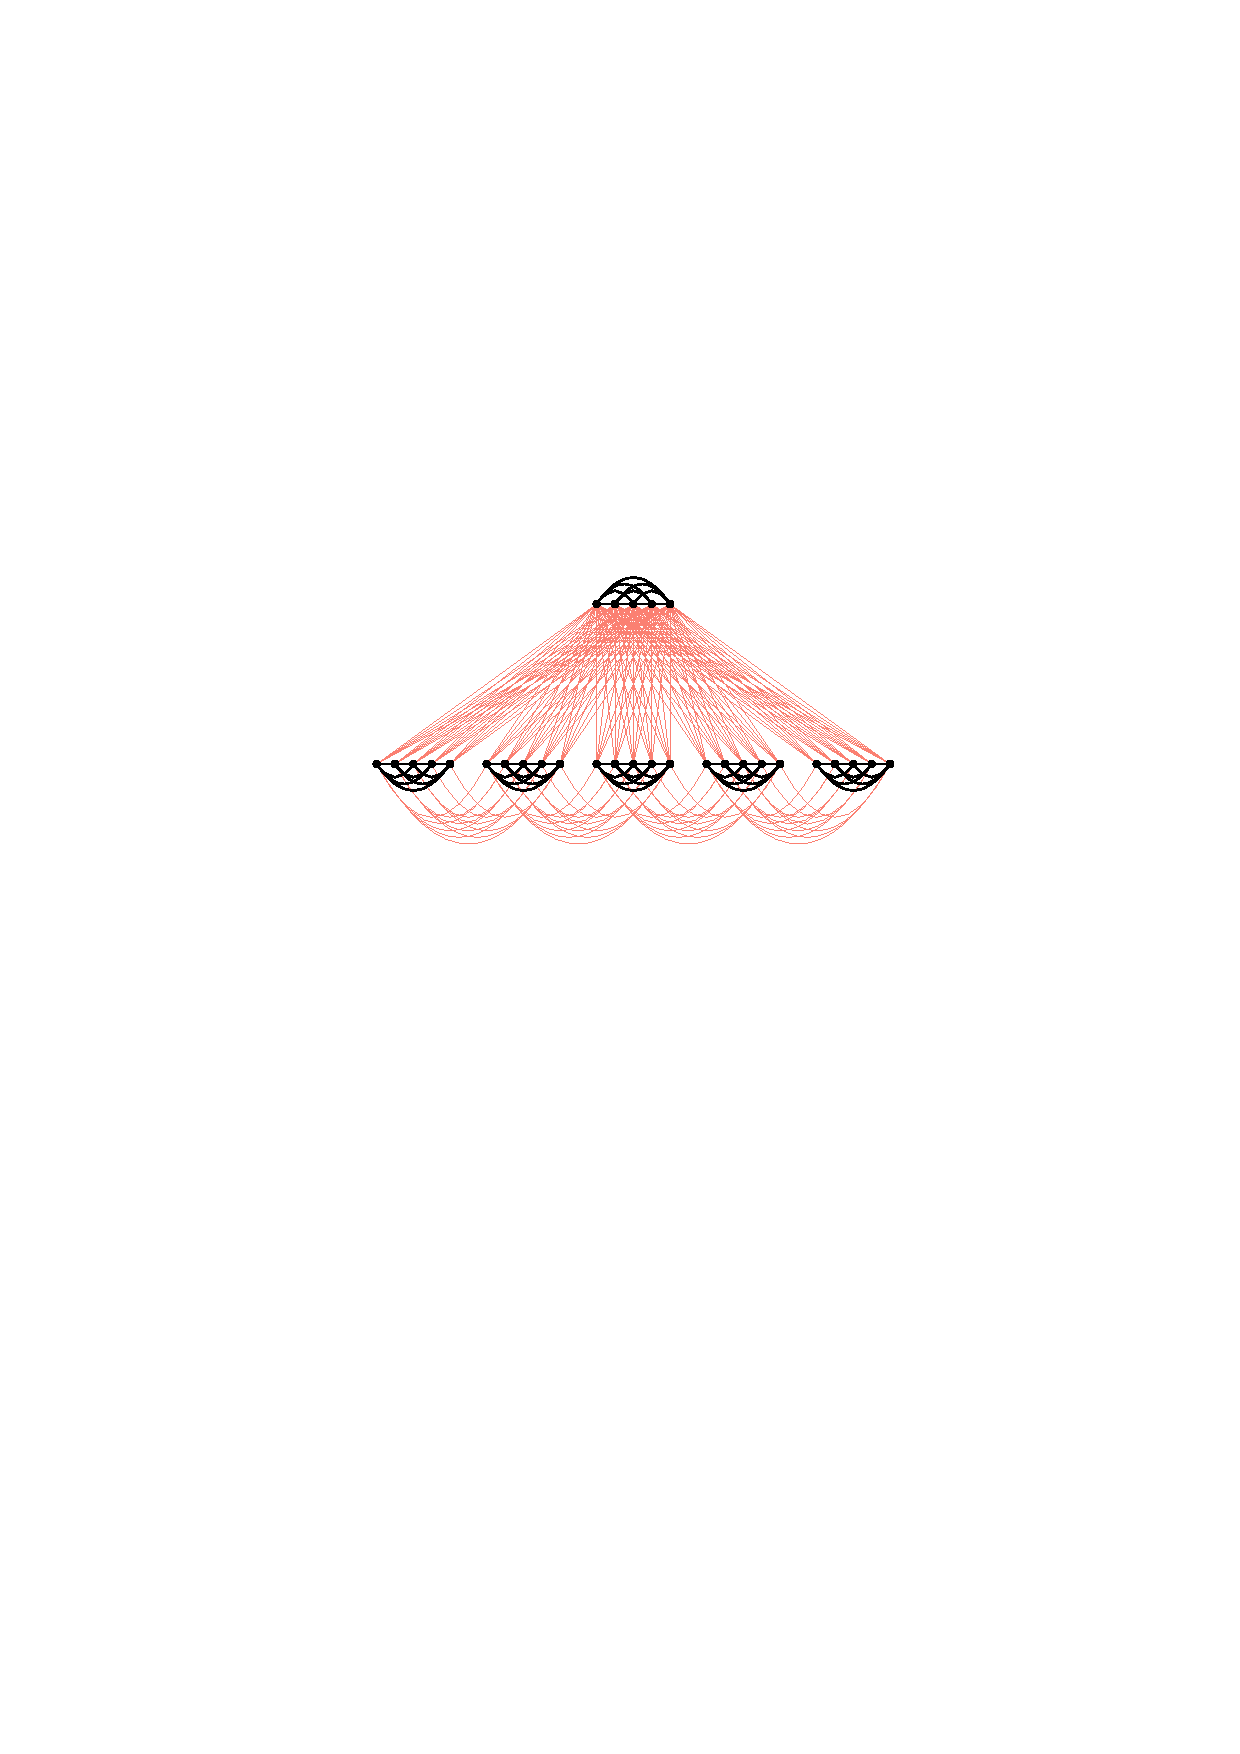
\includegraphics[width=.8\textwidth]{figs/fan-blowup}
  \end{center}
\end{frame}

\begin{frame}
  \frametitle{Path Partitions and Bandwidth}

  \uncover<1->{\textbf{Main Theorem:} Every $n$-vertex planar $G$ has a set $X$ of $\widetilde{O}(\sqrt{n})$ vertices such that $G-X$ has a \textcolor{red}{path partition} of width $\widetilde{O}(\sqrt{n})$}\\[2ex]

  \uncover<2->{\textbf{Main Theorem:} Every $n$-vertex planar $G$ has a set $X$ of $\widetilde{O}(\sqrt{n})$ vertices such that $G-X$ has a \textcolor{red}{bandwidth} $\widetilde{O}(\sqrt{n})$}

  \begin{center}
    \includegraphics[width=.8\textwidth,page=2]{figs/fan-blowup-slides}
  \end{center}

\end{frame}

\begin{frame}
  \frametitle{Obstacles to Small Bandwidth}

  \begin{tabular}{lr}
    \only<1>{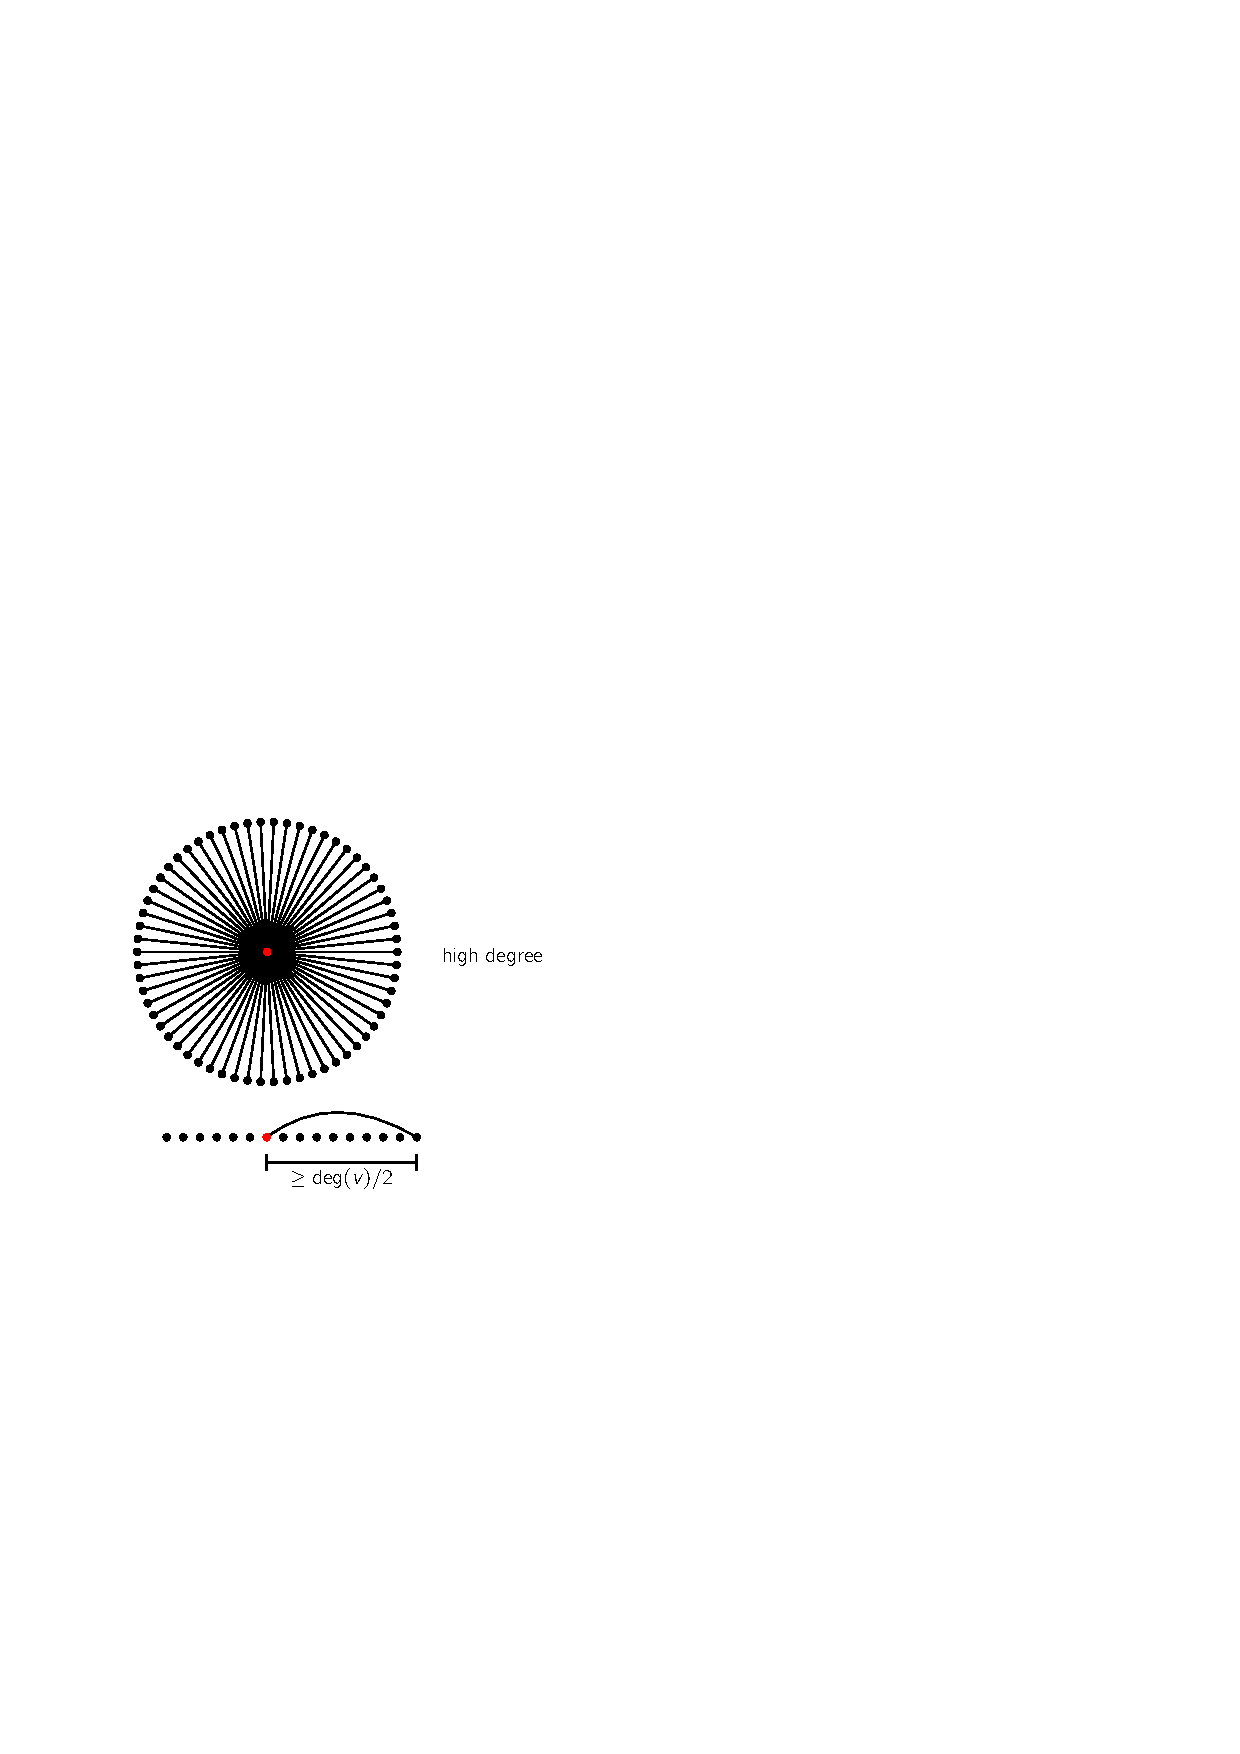
\includegraphics[page=1]{figs/bandwidth-obstacles}}%
    \only<2>{\includegraphics[page=2]{figs/bandwidth-obstacles}}%
    \only<3>{\includegraphics[page=3]{figs/bandwidth-obstacles}}%
    \only<4>{\includegraphics[page=4]{figs/bandwidth-obstacles}}% &
    \raisebox{5cm}{\includegraphics[width=.2\textwidth,page=2]{figs/fan-blowup-slides}}
  \end{tabular}
\end{frame}

\begin{frame}
  \frametitle{Local Sparsification}

  \textbf{Theorem (Feige 2000):} If $G-X$ has local density $\widetilde{O}(\sqrt{n})$ then $G$ has bandwidth $\widetilde{O}(\sqrt{n})$.\\[3ex]

  \only<2->{Find $X\subseteq V(G)$ of size $\widetilde{O}(\sqrt{n})$ so that every $r$-ball in $G-X$ contains $\widetilde{O}(r\sqrt{n})$ vertices.}
\end{frame}

\begin{frame}
  \frametitle{Local Sparsification}

  \only<1>{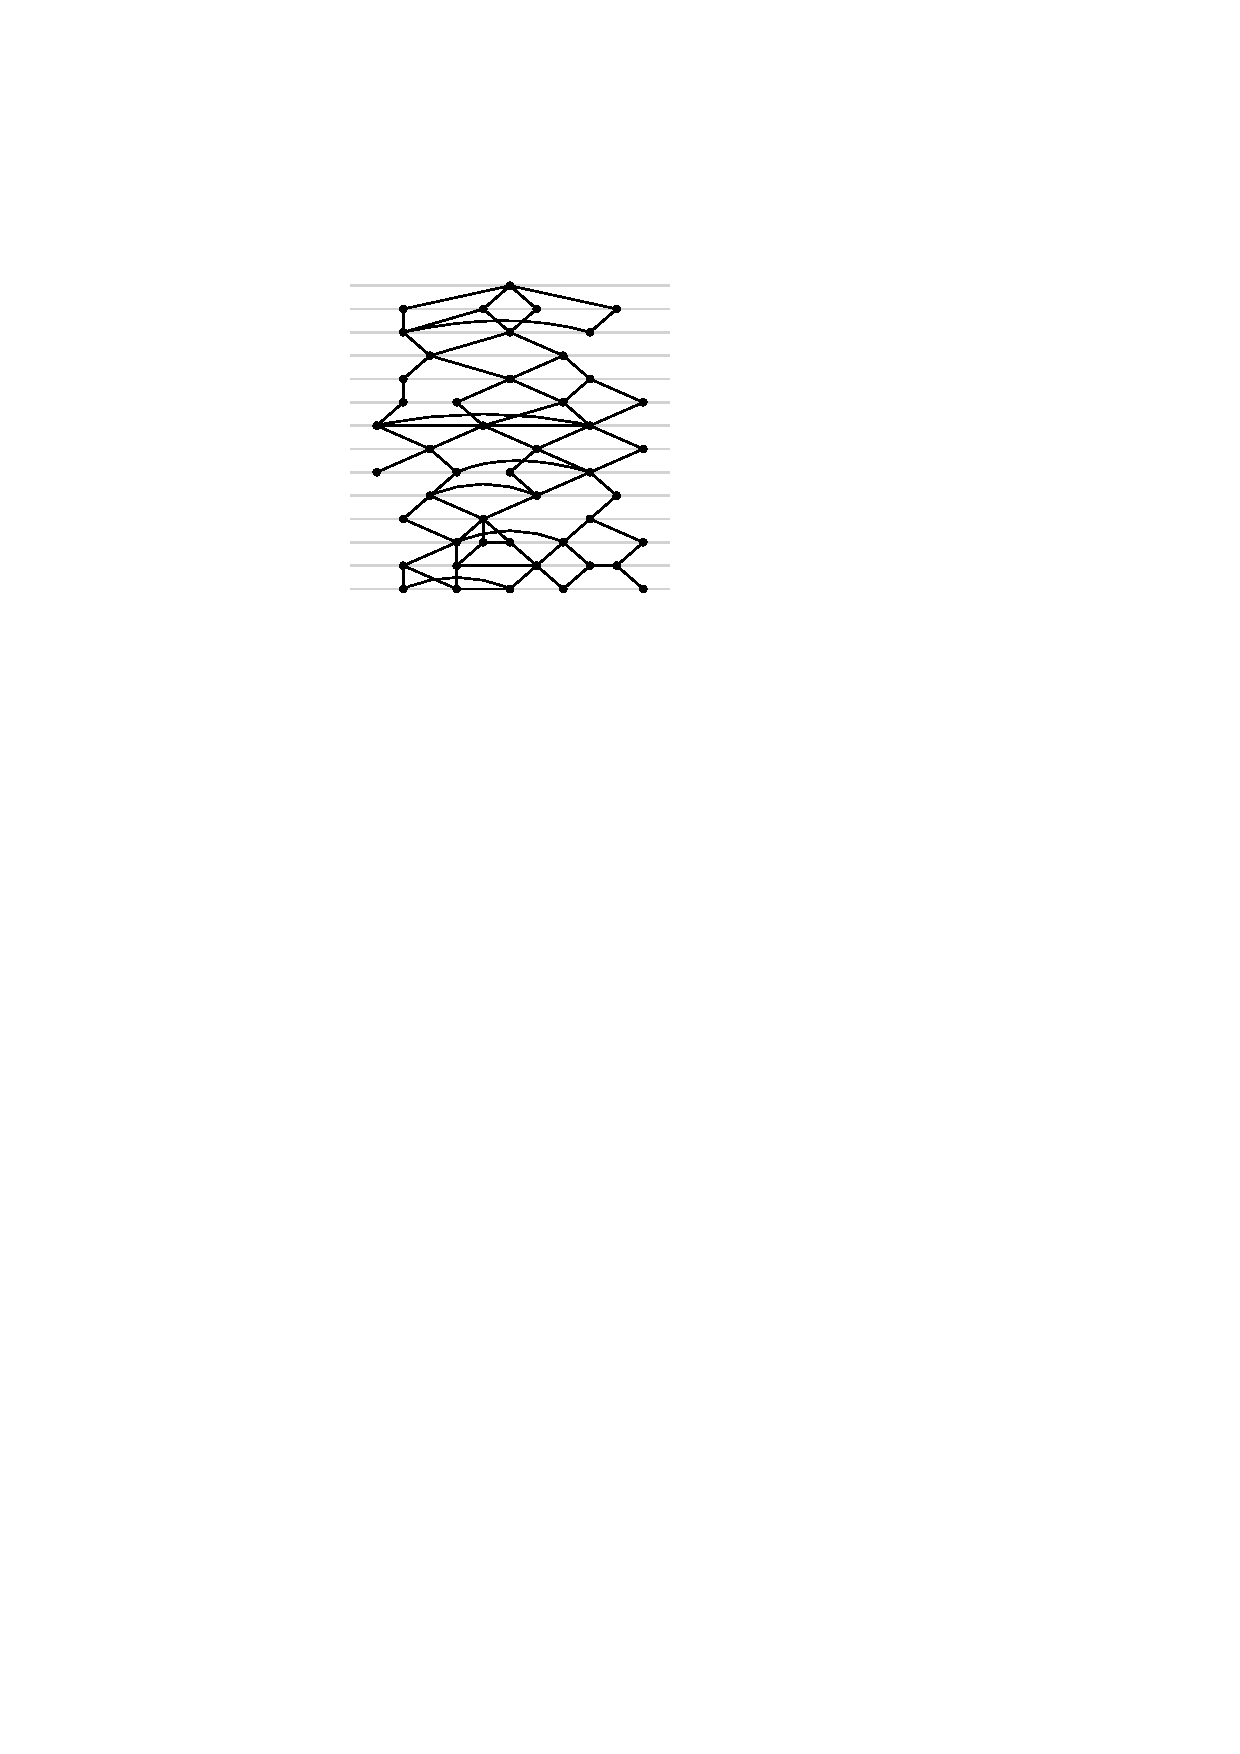
\includegraphics[page=1]{figs/layering}}%
  \only<2>{\includegraphics[page=2]{figs/layering}}%
  \only<3>{\includegraphics[page=3]{figs/layering}}%
  \only<4>{\includegraphics[page=4]{figs/layering}}%
  \only<5>{\includegraphics[page=5]{figs/layering}}%
  \only<6>{\includegraphics[page=6]{figs/layering}}%
  \only<7>{\includegraphics[page=7]{figs/layering}}%
  \only<8>{\includegraphics[page=8]{figs/layering}}%
  \only<9>{\includegraphics[page=9]{figs/layering}}%
  \only<10>{\includegraphics[page=10]{figs/layering}}%
\end{frame}

\begin{frame}
  \frametitle{Other Stuff}

  Same results hold for broader graph classes:\\[2ex]

  \only<2->{$k$-planar, bounded genus, $(g,k)$-planar, apex-minor-free, \newline \textcolor{red}{product structured}} \\[2ex]

  \only<3->{\textbf{Theorem (Distel 2024):} Every $K_t$-minor-free $G$ has a fan-partition of width $\widetilde{O}_t(\sqrt{n})$.}\\[3ex]

  \only<4->{\Huge\bf Thank You!}

\end{frame}


\end{document}

\end{document}
